\chapter{関係データモデル}

\strong{関係データベース(relational database)} とは,関係データモデルにもとづき表現されたデータの集まりである.
前章で述べたように,関係データモデルとは,表によってデータを表現するデータモデルである.
一見すると単純な表にしか見えない関係データモデルは数学によって定式化されており,強固な理論的基盤を有している.
関係データモデルを用いることで,データから冗長性を排除し,データを正しく管理することが可能となる.

以下では,数学的な観点から関係データモデルについて述べる.
少々堅い説明にはなるが,関係データベースという計算機科学技術が数学に支えられていることを知るためにも,眠気を我慢して読んでほしい.
なお,本講では数学における「集合と写像」の知識を使う.
%最低限の知識を[コチラ](../misc/math.md)にまとめたので,不安がある方はそちらを参照されたい.


\begin{notebox}{計算機科学とは抽象化の学問}
計算機科学(あるいは情報科学)というと「プログラミングでしょ」と考える学生は多いが,それは間違いである.
計算機科学の本質は,\strong{物事を計算可能な状態にする(抽象化)し,計算機の上で処理・分析}することにある.
データベースもその一つである.
計算機科学は抽象化の学問なのである.
\end{notebox}

% ---------------------------------------
\section{関係データモデルのデータ構造}
% ---------------------------------------
\begin{table}[tb]
\centering
\caption{ある小売店の商品に関するデータを収めた関係}
\label{tab:correct-table}
\begin{tabular}{@{}llll@{}}
商品            &             &             &              \\ \midrule
\textbf{商品ID} & \textbf{名称} & \textbf{単価} & \textbf{登録日} \\ \midrule
P1            & はーいお茶       & 130         & 2020/07/15   \\
P2            & 午前の紅茶       & 130         & 2020/09/25   \\
P3            & 健康麦茶        & 150         & 2021/02/16   \\
$\vdots$      & $\vdots$    & $\vdots$    & $\vdots$     \\
P1000         & きのこの里       & 200         & 2023/01/08   \\ \bottomrule
\end{tabular}
\end{table}

表\ref{tab:correct-table}は,ある小売店で取り扱っている商品のデータを関係データモデルによって表現したものである.
この表において,各行は小売店で取り扱っている商品に対応し,各列には各商品に関するデータが記述されている.

表の左上にある「商品」はこの表の名前を示しており,\strong{関係名}と呼ばれる.
関係データモデル上では,各行は\strong{タプル(tuple)} と呼ばれる.
表の1行目には,「商品」がどのようなデータを持つかを示す見出しが付けられている.
表における各見出しに対応するものを,関係データモデルでは\strong{属性(attribute)}と呼ぶ.
また,各タプルにおけるある属性の値を\strong{属性値}と呼ぶ.
例えば,表中の2行目に対応するタプルは
\begin{equation}
(``P1", ``はーいお茶", 130, ``2020/07/15")
\end{equation}
であるが,このタプルの属性「単価」の属性値は\graybox{130}となる.

% ---------------------------------------
\subsection{数学における「関係」}
% ---------------------------------------
ところで,関係データベースあるいは関係データモデルの「関係」とは一体何だろうか.
\strong{関係(relation)} とは数学上の概念である.
集合$S_1, S_2, ..., S_n$が与えられたとき,それらの直積集合$S_1 \times ... \times S_n$とは

\begin{equation}
S_1 \times ... S_n = \{(x_1, ..., x_n) \ | \ x_1 \in S_1, ..., x_n \in S_n \}
\end{equation}
と表現されるものである.
(数学上の概念である)関係とは,このような直積集合の部分集合を意味する.
正確に書くと,集合$S_1, S_2, ..., S_n$が与えられたとき,直積集合$S_1 \times ... \times S_n$の部分集合を$S_1, S_2, ..., S_n$上の\strong{n項関係}と呼ぶ.

例えば,$A=\{2, 3\}$,$B=\{-2, -3\}$が与えられたとき,直積$A \times B$は集合AおよびBの要素のすべての組み合わせであるから

\begin{equation}
A \times B = \{(2, -2), (2, -3), (3, -2), (3, -3)\}
\end{equation}
となる.
このとき,その部分集合の1つである
\begin{equation}
\{(2, -3), (3, -2)\}
\end{equation}
は集合AおよびB上の2項関係となる.
このような(n項)関係の概念を使って,関係データモデルは理論構築されている


% ---------------------------------------
\subsection{関係データモデルにおける「関係」}
% ---------------------------------------
\strong{関係データモデルにおける関係}は「数学におけるの関係」を拡張したものになっており,以下の2つから構成される.
\begin{itemize}
\item 関係スキーマ
\item インスタンス
\end{itemize}

\strong{関係スキーマ(relation schema)} とは,関係の名前と属性の集合,および(後述する)一貫性制約の情報を示すものである.
関係スキーマは

\begin{equation}
(\boldsymbol{R}(A_1, ..., A_n), \{\sigma_1, \sigma_2, ..., \sigma_m\})
\end{equation}
の形式で記述される.
ここで
\begin{itemize}
\item $\boldsymbol{R}$は関係名
\item $A_1, ..., A_n$は属性
\item $\sigma_1, ..., \sigma_m$は一貫性制約
\end{itemize}
に対応する.
一貫性制約が自明な場合やそれを考慮しないときは,関係スキーマを

\begin{equation}
\boldsymbol{R}(A_1, ..., A_n)
\end{equation}
のように簡潔に表記することもある.
表\ref{tab:correct-table}の関係「商品」の例の場合,関係スキーマは
\begin{equation}
商品(商品ID, 名称, 単価, 登録日)
\end{equation}
と記述する.

関係スキーマに記された各属性には,属性が取り得る値の集合を定義する.
この集合は\strong{ドメイン(domain; 定義域)} と呼ばれ,属性$A$のドメインは$Dom(A)$と記す.
例えば,表\ref{tab:correct-table}の関係「商品」の例では,属性「単価」は金額を表すので,そのドメイン$Dom(単価)$は0以上の整数値が想定される.
これを数学的に記すと,以下のようになる:
\begin{equation}
Dom(単価) = \{ x \ | \ x \in \mathbb{N} \}
\end{equation}

同様に,属性「商品ID」「名称」「登録日」についても,以下のようにドメインを定義できる.
\begin{eqnarray}
Dom(商品ID) = \{ x \ | x \in Pから始まる文字列集合 \} \\
Dom(名称) = \{ x \ | \ x \in 文字列集合 \} \\
Dom(登録日) = \{ x \ | \ x \in 年月日集合(ただし西暦表記) \}
\end{eqnarray}

\strong{インスタンス(instance)} は,関係スキーマ$\boldsymbol{R}(A_1, ..., A_n)$におけるドメイン$Dom(A_1), ..., Dom(A_n)$の直積の部分集合である.
仮にインスタンスを$R$とすると,
\begin{equation}
R \subset{Dom(A_1) \times ... \times Dom(A_n)}
\end{equation}
である.
インスタンスは,前節で説明した数学上の関係に相当する.
また,インスタンス$R$の要素がタプルとなる.

例に戻って,定義と照らし合わせてみよう.
表\ref{tab:correct-table}の関係「商品」の関係スキーマは$商品(商品ID, 名称, 単価, 登録日)$であった.
各属性のドメインの定義も与えたが,その定義から,例えば属性「単価」については
\begin{equation}
Dom(単価) = \{1, 2, 3, .... 10000, .... \}
\end{equation}
のようにあらゆる自然数を取り得る.
また,属性「名称」については
\begin{equation}
Dom(名称) = \{``あ", ``い", ..., ``はーいお茶", ... \}
\end{equation}
のようにあらゆる文字列を取り得る.

各属性の直積$Dom(商品ID) \times Dom(名称) \times Dom(単価) \times Dom(登録日)$には,
\begin{equation}
(``P001", ``こんな商品はありません", 100兆, ``2020/01/01")
\end{equation}
のように,実際に商品情報としてありえないタプルも含めて,様々なタプルが要素として含まれる.
なぜなら,直積とは集合(ドメイン)の要素のすべての組み合わせであるためである.
ドメインの直積の部分集合をインスタンスとすることは,取り得るタプルの候補から実際にデータとして扱われるタプルの集合を選択することに相当する.


\begin{notebox}{タプルは重複が許されない}
一般的に使われる表では,同じ内容を表す行が複数あっても許される.
一方,関係データモデルに基づく表は行,すなわちタプルの重複は許されない.
なぜなら,関係データモデルのインスタンスは(数学的な)集合だからである.
\end{notebox}


% ---------------------------------------
\section{非正規関係と第1正規形}
% ---------------------------------------
関係データモデルにおけるドメインとは属性が取り得る値の集合を意味するが,ドメインの要素はそれ以上分解不可能な値を意味する\strong{原子値(atomic value)} であることを想定している.
原子値の例としては,文字列,整数,実数,真偽値,日付などが挙げられ,どれもデータの基本単位と呼べるものである.
逆に原子値で「ない」例としては,タプルや集合,関係などが挙げられる.
ドメインとして原子値以外の値をとることを許す関係データを\strong{非正規関係(unnormalized relation)} と呼ぶ.
逆に,ドメインとして原子値しかとらない関係は\strong{第1正規形(first normal form; 1NF)である} という.

\begin{figure}[tb]
    \centering
    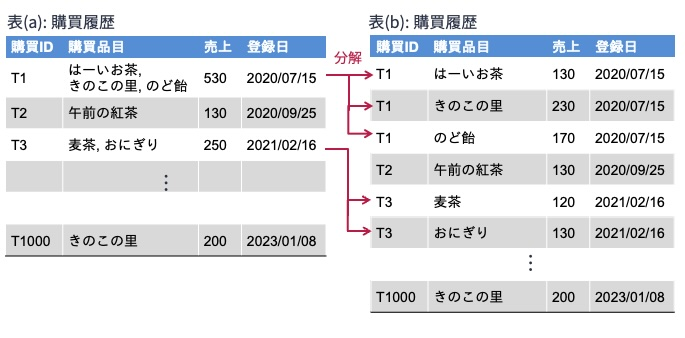
\includegraphics[width=1.0\textwidth]{figure/unnormalized-relation.jpg}
    \caption{非正規関係}
    \label{fig:unnormalized-relation}
\end{figure}

例えば,図\ref{fig:unnormalized-relation}の(a)(b)はともに商品の購買履歴を表しているが,(a)は属性「購入品目」に集合要素が入ってしまっている(例えば,\graybox{\{``はーいお茶'', ``きのこの里'', ``のど飴''\}}).
(a)の属性「購入品目」のドメインが原子値以外の値(つまり文字列の集合)を許してしまっていることから,(a)は非正規関係と見なせる.

一方,図\ref{fig:unnormalized-relation}(b)は(a)の購買品目の値が原子値(文字列の集合ではなく文字列)になるように設計されているため,第1正規形と見なせる.
図\ref{fig:unnormalized-relation}(a)では1行で表現できていた1回分の購買データが,(b)では複数行を使って表現されている.
図\ref{fig:unnormalized-relation}(b)のほうがデータ構造が簡潔になるため,データが扱いやすい.


% ---------------------------------------
\section{一貫性制約}
% ---------------------------------------
\strong{一貫性制約(integrity constraint)} とは,データベースが対象とする実世界を反映するように設定された,データが満たすべき規則である.
関係データモデルにおいては,代表的な一貫性制約として以下がある:
\begin{itemize}
\item ドメイン制約
\item キー制約
\item 参照制約
\item データ従属性
\end{itemize}

関係データモデルを扱うデータベースを設計する際には,上記一貫性制約を踏まえて\strong{関係スキーマの定義や(複数の関係スキーマへの)分解} を行う.


% ---------------------------------------
\subsection{ドメイン制約}
% ---------------------------------------
\strong{ドメイン制約(domain constraint)} とは,関係$\boldsymbol{R}(A_1, ..., A_n)$に含まれるタプルの各成分は,対応する属性のドメインの要素でなければならならいという制約である.
これは属性の定義ですでに触れたことである.
ドメイン制約では,各属性のドメインのデータ型(例: 整数,実数,文字列,日付)に加えて,値が取り得る範囲を指定することもある.
例えば,

先の例でとりあげた関係
\begin{equation}
商品(商品ID, 名称, 単価, 登録日)
\end{equation}
において,属性「単価」や「登録日」のドメインは
\begin{eqnarray}
Dom(単価) = \{ x \ | \ x \in \mathbb{N} \} \\
Dom(登録日) = \{ x \ | \ x \in 年月日集合(ただし西暦表記) \}
\end{eqnarray}
のように定義されていた.
これらはドメイン制約である.
これら制約にもとづき,
\begin{itemize}
\item 「単価」属性の値は\strong{必ず}自然数
\item 「登録日」属性の値は\strong{必ず}西暦表記の年月日集合
\end{itemize}
でなければならない.
よって,表\ref{tab:incorrect-table}に記した表「商品(*)」の各タプルは関係「商品(商品ID, 名称, 単価, 登録日)」のインスタンスには\strong{なれない}.
なぜなら,
\begin{itemize}
\item 商品IDがP1の商品の登録日は年月はあるが日が抜けている
\item 商品IDがP3の商品の登録日は和暦で表現されている
\item 商品IDがP1000の商品の単価は漢数字(文字列)で表現されている
\end{itemize}
からである.

\begin{table}[tb]
\centering
\caption{ドメイン制約に違反する関係}
\label{tab:incorrect-table}
\begin{tabular}{@{}llll@{}}
商品(*)            &             &             &              \\ \midrule
\textbf{商品ID} & \textbf{名称} & \textbf{単価} & \textbf{登録日} \\ \midrule
P1            & はーいお茶       & 130         & 2020/07   \\
P2            & 午前の紅茶       & 130         & 2020/09/25   \\
P3            & 健康麦茶        & 150         & 令和3年2月16日   \\
$\vdots$      & $\vdots$    & $\vdots$    & $\vdots$     \\
P1000         & きのこの里       & 2百         & 2023/01/08   \\ \bottomrule
\end{tabular}
\end{table}


% ---------------------------------------
\subsection{キー制約}
% ---------------------------------------
まず,キー制約の前提となるキーの概念について説明する.
関係$\boldsymbol{R}$における\strong{超キー(super key)} とは,関係$\boldsymbol{R}$における属性の集合のうち,それらの属性値が決まればおのずと関係$\boldsymbol{R}$のタプルが唯一ひとつに決まる(タプルを一意に特定できる)ものを指す.

例えば,表\ref{tab:contact-relation}は関係スキーマ
\begin{equation}
連絡先(学生ID, 名前, 学年, 大学email, 自宅住所)
\end{equation}
に従うデータを表形式で記したもので,各行(タプル)は学生の連絡先情報を示している.
大学において学生情報を管理する場合,学生ID(の値)が決まれば唯一ひとつの学生連絡先情報(行; タプル)を照会できるよう,学生IDは重複がないように設定される.
それゆえ,この関係「連絡先」において属性「学生ID」は超キーとなる.
同様に,属性「大学email」も超キーとなる.

なお,\{ 学生ID, 名前 \},\{ 学生ID, 名前, 学年 \} のように学生IDを含む属性の集合も超キーになる.
例えば,「学生ID」が\graybox{S1},「名前」が\graybox{川澄桜}である行は唯一1行に決まるので,属性集合 \{ 学生ID, 名前 \} も超キーになる.
これは属性「学生ID」が超キーであるから,当たり前である.

一方,属性「住所」は超キーにはなり得ない.
学生IDが\graybox{S3}と\graybox{S4}の学生の住所が同じ(つまり同じところに住んでいる)であるから,住所を1つ指定しても連絡先タプルが一意に特定できないからである.


\begin{table}[tb]
\centering
\caption{関係「連絡先」}
\label{tab:contact-relation}
\begin{tabular}{@{}lllll@{}}
連絡先           &             &             &                    &               \\ \midrule
\textbf{学生ID} & \textbf{名前} & \textbf{学年} & \textbf{大学email}   & \textbf{自宅住所} \\ \midrule
S1            & 川澄 桜        & 4           & kawasumi@xxx.ac.jp & 名古屋市xxx       \\
S2            & 山畑 滝子       & 3           & taki@xxx.ac.jp     & 岡崎市xxx        \\
S3            & 田辺 通        & 3           & t.tanabe@xxx.ac.jp & 尾張旭市xxx       \\
S4            & 田辺 瑞穂       & 1           & m.tanabe@xxx.ac.jp & 尾張旭市xxx       \\
$\vdots$      & $\vdots$    & $\vdots$    & $\vdots$           & $\vdots$      \\
S1000         & 北 千種        & 2           & kita@xxx.ac.jp     & 名古屋市xxx       \\ \bottomrule
\end{tabular}
\end{table}


超キーは複数ありえるが,上の例では属性「学生ID」のみでタプルを特定できるように,属性集合 { 学生ID, 名前 } を使ってタプルを特定しようとするのは無駄であろう.
そこで,超キーのうち極小(つまり最も小さい部分集合)のものを\strong{候補キー(candiate key)} と定義する.
候補キーは単純に\strong{キー(key)} と呼ばれることもある.
例えば,上の関係「連絡先」では,属性「学生ID」や「大学email」が候補キーとなりえる.

最後に\strong{主キー(primary key)} の概念を導入する.
候補キーのうち,値として\strong{未定義や空の値(空値またはNULL値と呼ばれる)} を取る可能性がなく,かつデータベース管理上都合のよいキーの1つを主キーと決める.
主キー以外の候補キーは\strong{代替キー}と呼ばれる.
例えば,先の関係「連絡先」の場合,候補キーは「学生ID」と「大学email」であったが,大学emailは「氏名\@xxx.ac.jp」のようなものから「学籍番号\@xxx.ac.jp」のようなものに変更される可能性があったとしても,学生IDは一度決めたらほぼ変わらないと思われる.
これらを鑑みると,関係「連絡先」においては属性「学生ID」を主キーとして選ぶのがよさそうである.

なお,候補キーの定義から主キーは属性の集合をとることができる.
このような主キーを\strong{複合主キー(composite primary key)} と呼ぶ.
例えば,表\ref{tab:course-completion-relation}は,学生が履修した科目の成績をあらわす関係「履修」を表にしたものである.
この表においては科目IDあるいは学生IDだけでは成績が特定できないが,科目IDと学生IDの両方が決まれば,ある学生のある科目の成績が特定される.
それゆえ,関係「履修」においては \{ 科目ID, 学生ID \} の属性ペアが主キーとなる.

\begin{table}[tb]
\centering
\caption{関係「履修」}
\label{tab:course-completion-relation}
\begin{tabular}{@{}lll@{}}
履修            &               &             \\ \midrule
\textbf{科目ID} & \textbf{学生ID} & \textbf{成績} \\ \midrule
C1            & S1            & 不可          \\
C2            & S1            & 良           \\
C2            & S2            & 優           \\
C3            & S3            & 可           \\
$\vdots$      & $\vdots$      & $\vdots$    \\ \bottomrule
\end{tabular}
\end{table}

関係表と主キー,候補キー,超キーの関係は,図\ref{fig:key-concept-mapping}のようにまとめることができる.
\begin{figure}[tb]
    \centering
    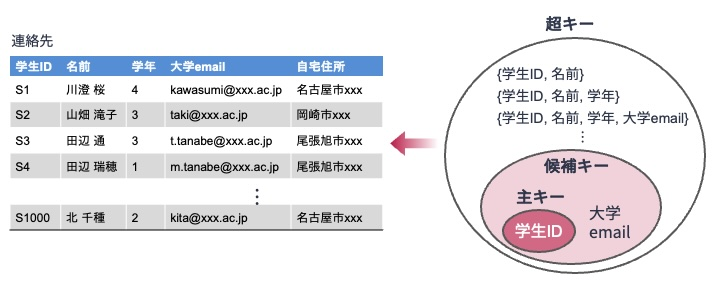
\includegraphics[width=1.0\textwidth]{figure/key-concept-mapping.jpg}
    \caption{キーの概念の整理}
    \label{fig:key-concept-mapping}
\end{figure}

ここまで,超キー,候補キー,主キーの説明を行ったが,最後に本節の主題であるキー制約について述べる.
\strong{キー制約(key constraint)} は,関係$\boldsymbol{R}$の関係スキーマに対して主キーが設定されたとき,$\boldsymbol{R}$のインスタンスにおいて
\begin{itemize}
\item 主キーに設定された属性の値は重複があってはならない,かつ
\item その要素(タプル)は主キーによって一意に特定されなければならない,かつ
\item 主キーとなる属性の値は\strong{NULL値} であってはならない
\end{itemize}
という制約である.
定義は小難しく見えるかもしれないが,キー制約は「ある属性が主キーと設定されたら,それがきちんと主キーの役割を果たすようデータが作られなければならない」ということを意味している.
主キーを定義できれば,キー制約を定義できたようなものである.

さて,関係スキーマにおいてキー制約以外の一貫性制約には注目しない場合,関係スキーマでは主キーは以下のように下線を引いて表す.
\begin{equation}
\boldsymbol{R}(\underline{A_1, A_2}, ..., A_n)
\end{equation}
例えば,図\ref{fig:key-concept-mapping}の関係「連絡先」であれば,その関係スキーマは以下のように表す.
\begin{equation}
連絡先(\underline{学生ID}, 名前, 学年, 大学email, 自宅住所)
\end{equation}

\begin{notebox}{キーは関係スキーマに対して設定される}
キーは,関係データベース内にあるタプル(行)だけを見て決めてはいけない.
例えば表\ref{tab:contact-relation}に示した関係「連絡先」の場合,表の見えているところだけに注目すると,属性「名前」もキーに見える.
しかし,現実的には同性同名の学生が存在しうる.
そのため,「名前」をキーにすると,連絡先のタプルを一意に特定できない可能性が生じる(キーの性質を失う).

そもそも関係データモデルにおいては,どのようなデータをデータベースに格納する可能性があるかを事前に想定して関係スキーマを設定する(その中にキーの設定も含まれる).
その上で,設定した関係スキーマに従ってデータを生成し格納する.
決してインスタンスを見てキーを決めるわけではない.
キーは「\strong{関係スキーマに対して設定される}」ことを意識しよう.
\end{notebox}


% ---------------------------------------
\subsection{参照整合性制約}
% ---------------------------------------
(関係データモデルにもとづく)関係データベースでは,対象となる事象のデータを正しく管理するために,\strong{データを複数の関係(表)で管理する}ことがほとんどである.
複合主キーの説明の例で使った関係「履修」(表\ref{tab:course-completion-relation}参照)には,その値だけ見ても具体的に何を意味しているのかが分からない属性「科目ID」「学生ID」がある.
これらの意味を読み解くためには
\begin{itemize}
\item 「科目ID」がどのような科目のことを指しているのか
\item 「学生ID」がどの学生のことを指しているのか
\end{itemize}
といった情報を管理する他の関係(表)が必要となる.
図\ref{fig:score-db}は,学生の成績を管理するための関係データベースの例である.
この中には関係「履修」も含まれている.
\begin{figure}[tb]
    \centering
    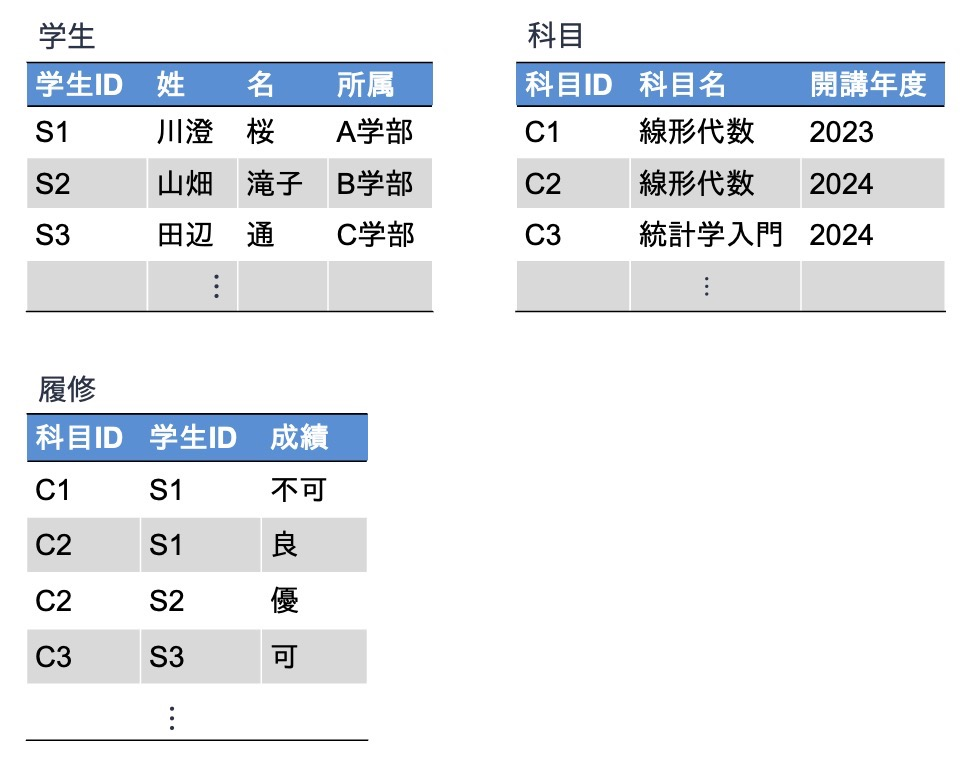
\includegraphics[width=1.0\textwidth]{figure/score-db.jpg}
    \caption{成績管理データベース}
    \label{fig:score-db}
\end{figure}
図中の3つの関係(表)があれば,
\begin{itemize}
\item 関係「学生」から「学生ID」が\graybox{S1}のものを探し,
\item 関係「科目」から「科目ID」が\graybox{C1}のものを探す
\end{itemize}
ことで,関係「履修」において「学生ID」が\graybox{S1}で「科目ID」が\graybox{C1}の「成績」が\graybox{不可}だった件について,具体的にどんな学生が何の科目を落としてしまった(不可になってしまった)かを把握することができる.
このとき,関係「履修」のタプルにある「科目ID」の\graybox{C1}という値が,関係「科目」のインスタンスの属性「科目ID」に含まれていなければならない(関係「科目」の科目IDの列にその値が存在しなければならない),ということは自明であろう.
関係「履修」の中にはあるが,関係「科目」には存在していなければ,データ管理として破綻していることになる.
「学生ID」の\graybox{S1}についても同様である.

上記の例では,
\begin{itemize}
\item 関係「履修」の属性「学生ID」は関係「学生」の主キーである「学生ID」と
\item 関係「履修」の属性「科目ID」は関係「科目」の主キーである「科目ID」と
\end{itemize}

紐付いていることが分かる.
言い方を変えると,関係「履修」は属性「学生ID」および「科目ID」の値を通して,関係「学生」および「科目」の情報を参照していることになる.

このように,関係スキーマ$\boldsymbol{R_1}(..., FK, ...)$と$\boldsymbol{R_2}(\underline{PK}, ...)$が与えられ,$\boldsymbol{R_1}$におけるタプルの属性$FK$の値は必ず$\boldsymbol{R_2}$におけるいずれかのタプルの主キー$PK$の値と一致するように設計されているとき,$\boldsymbol{R_1}$の属性$FK$を$\boldsymbol{R_2}$の$PK$に対する\strong{外部キー(foreign key)} と呼ぶ.
関係スキーマ上では,関係$\boldsymbol{R_1}$の属性$FK$が関係$\boldsymbol{R_2}$の主キー$PK$に対する外部キーであることを以下のように記す.
\begin{equation}
\boldsymbol{R_1}.FK \subseteq \boldsymbol{R_1}.PK
\end{equation}

図\ref{fig:score-db}の例では,関係「履修」の属性「学生ID」および「科目ID」が外部キーとなるので,関係スキーマとして
\begin{eqnarray}
履修.学生ID \subseteq 学生.学生ID \\
履修.科目ID \subseteq 科目.科目ID
\end{eqnarray}
と記す.

前置きが長くなったが,本節のテーマである\strong{参照整合性制約(referential constraint)} とは「関係スキーマにおいて外部キーが設定されたとき,そのいかなるインスタンスも設定された外部キーの条件を満たさなければいけない」という制約である.

% ---------------------------------------
\subsection{データ従属性}
% ---------------------------------------
一貫性制約として,ドメイン制約,キー制約,参照制約を挙げてきた.
関係データモデルにはこれら以外にも,データ間に成立する制約を数学的に記述する手段がある.
これを\strong{データ従属性(data dependency)} と呼ぶ.

データ従属性としては,関数従属性,多値従属性,結合従属性など,様々なものが提案されている.
\strong{関数従属性(functional dependency)} は,データ従属性の中でも最も単純で,かつ実用的なものである.
関数従属性は,「関係$\boldsymbol{R}(..., X, ..., Y, ...)$において,属性(あるいは属性集合)$X$の値が決まると属性$Y$の値も一意に決まる」という性質である.
このことを
\begin{equation}
X \to Y
\end{equation}
と記す.

例えば,関係として
\begin{equation}
連絡先(\underline{学生ID}, 名前, 学年, 大学email, 郵便番号, 都道府県, 自宅住所)
\end{equation}
が与えられたとしよう.
一般常識から,住所が決まればそれが存在する都道府県や郵便番号もひとつに決まる.
このことから,関係「連絡先」においては
\begin{eqnarray}
自宅住所 \to 郵便番号 \\
自宅住所 \to 都道府県
\end{eqnarray}
という関数従属性が定義できる.
関数従属性はキー制約を一般化したものと捉えることができる.

データ従属性は,データの更新があったときにその影響が最小限になるように関係データベースを設計する上で,極めて重要である.
それゆえ,特に関数従属性については別章で取り上げる.


% ---------------------------------------
\section{クイズ}
% ---------------------------------------
\subsubsection{Q1. 直積}
集合$S_{lang}$,$S_{popularity}$,$S_{difficulty}$を以下のように定義する:
\begin{eqnarray}
S_{lang} = \{Python, R, C^{++}\} \\
S_{popularity} = \{人気, 不人気\} \\
S_{difficulty} = \{難, 普通, 易\}
\end{eqnarray}
このとき,直積集合$S_{lang} \times S_{popluarity} \times S_{difficulty}$の要素をすべて列挙せよ.

\subsubsection{Q2. 関係}
Q1で定義した集合$S_{lang}$,$S_{popularity}$,$S_{difficulty}$上の3項関係を適当に考えよ
(※ 正解は一意に決まらないので,深く悩まずクイズに取り組むこと).


\subsubsection{Q3. 関係スキーマ}
関係スキーマ
\begin{equation}
学生(\underline{学籍番号}, 氏名, 学部, 年齢, 出身都道府県)
\end{equation}
に従う表データの例を作成せよ.
なお,表の行数は見出し行を含めて5-6行程度でよい.


\subsubsection{Q4. ドメイン}
Q3で定義した関係スキーマ「学生」の各属性について,そのドメインを定義せよ.
\begin{equation}
Dom(学籍番号) = \{ ... \}
\end{equation}
の形式で頑張って書いてみること.

\subsubsection{Q5. ドメイン制約}
Q4で定義した関係スキーマ(ドメイン定義を含む)に対して,ドメイン制約に違反しているタプルの例を2,3個列挙せよ.


\subsubsection{Q6. 候補キー(令和4年度 ITパスポート試験 問65改題)}
関係スキーマ
\begin{equation}
従業員(従業員番号, 従業員名, 部門コード, 生年月日, 住所)
\end{equation}
において,候補キーは何か.
なお,関係「従業員」は以下のような制約条件をもつ:
\begin{itemize}
\item 各従業員は重複のない従業員番号を1つだけもつ
\item 同姓同名の従業員がいてもよい
\item 各部門は重複のない部門コードを1つだけもつ
\item 1つの部門には複数名の従業員が所属する
\item 1人の従業員が所属する部門は1つだけである
\end{itemize}


\subsubsection{Q7. 主キー}
表\ref{tab:membership-management}の「会員管理」において,想定される主キーは何か.

\begin{table}[tb]
\centering
\caption{関係「会員管理」}
\begin{tabular}{@{}lllll@{}}
会員管理 &            &             &               &               \\ \midrule
\textbf{店舗コード} & \textbf{店舗名} & \textbf{会員番号} & \textbf{会員名} & \textbf{会員種別} \\ \midrule
S01            & 星ヶ丘          & 1             & 山畑 滝子        & ゴールド          \\
S01            & 星ヶ丘          & 2             & 田辺 通         & ゴールド          \\
S02            & 八事           & 1             & 北 千種         & 学生            \\
S02            & 八事           & 2             & 川澄 桜         & プラチナ          \\
S02            & 御器所          & 1             & 川澄 桜         & 一般            \\ \bottomrule
\end{tabular}
\label{tab:membership-management}
\end{table}


\subsubsection{Q8. 参照整合性制約}
以下の関係スキーマをもつ5つの関係からなるデータベースにおいて,定義すべき参照整合性制約をあげよ.
\begin{eqnarray}
顧客(\underline{顧客ID}, 氏名, 性別) \\
店舗(\underline{店舗ID}, 店舗名, 住所) \\
商品(\underline{商品ID}, 商品名, 商品カテゴリID, 単価) \\
購買(\underline{購買ID}, 店舗ID, 顧客ID, 商品ID, 個数, 購買日) \\
商品カテゴリ(\underline{商品カテゴリID}, カテゴリ名)
\end{eqnarray}
